\section{The influence of feature templates on time complexity}
In shift-reduce parsing, the search space will be very large depending on the feature templates we used. Therefore, in this section, we would like to make some evaluation about the time complexity of feature templates and then design a feature template used for exact search in shift-reduce constituent parsing.

\subsection{Evaluation from the baseline feature template}
In \cite{ref:2009Zhang}, they has designed an efficient baseline feature template which is widely used for shift-reduce constituent parsing. The feature template can be viewed as in table \ref{baseline feat} as long as its components and sub-components has been shown in table \ref{baseline comp} and \ref{baseline subcomp}, respectively.

\begin{table*}[t]
	\caption{\label{baseline feat} A table of baseline feature template}
	\begin{center}
		\begin{tabular}{|l|l|}
			\hline 
			Description & Templates  \\ 
			\hline
			1-grams 	& $s_0.t+s_0.c$   ;   $s_0.w+s_0.c$ ; $s_1.t+s_1.c$   ;   $s_1.w+s_1.c$ \\
			& $s_2.t+s_2.c$   ;   $s_2.w+s_2.c$   ;   $s_3.t+s_3.c$   ;   $s_3.w+s_3.c$ \\
			& $q_0.w+q_0.t$   ;   $q_1.w+q_1.c$   ;   $q_2.w+q_2.t$   ;   $q_3.w+q_3.c$ \\
			
			& $s_0l.w+s_0l.c$   ;   $s_0u.w+s_0u.c$   ;   $s_0r.w+s_0r.c$ \\
			& $s_1l.w+s_1l.c$   ;   $s_1u.w+s_1u.c$   ;   $s_1r.w+s_1r.c$ \\
			\hline
			2-grams 	& $s_0.w+s_1.w$   ;   $s_0.w+s_1.c$   ;   $s_0.c+s_1.w$   ;   $s_0.c+s_1.c$ \\
			& $s_0.w+q_0.w$   ;   $s_0.w+q_0.t$   ;   $s_0.c+q_0.w$   ;   $s_0.c+q_0.t$ \\
			& $q_0.w+q_1.w$   ;   $q_0.w+q_1.t$   ;   $q_0.t+q_1.w$   ;   $q_0.t+q_1.t$ \\
			& $s_1.w+q_0.w$   ;   $s_1.w+q_0.t$   ;   $s_1.c+q_0.w$   ;   $s_1.c+q_0.t$ \\
			\hline
			3-grams 	& $s_0.c+s_1.c+s_2.c$   ;   $s_0.w+s_1.c+s_2.c$ ; $s_0.c+s_1.w+s_2.c$   ;   $s_0.c+s_1.c+s_2.w$ \\
			& $s_0.c+s_1.c+q_0.t$   ;   $s_0.w+s_1.c+q_0.t$   ;   $s_0.c+s_1.w+q_0.t$   ;   $s_0.c+s_1.c+q_0.w$ \\
			\hline
		\end{tabular}
	\end{center}
\end{table*}

To evaluate the time complexity of shift-reduce parsing system applying this feature template, we will reply on the observation that the baseline feature has focused on top four nodes in stack $S$ (table \ref{baseline comp}). With each node, we could consider the parsing process as a CYK process. As we know, dynamic algorithm such as CYK can parse an input sentence within $O(n^3.|G|)$ (cubic time) with unlexicalized case and $O(n^5.|G|)$ with lexicalized case. The table \ref{baseline subcomp} has shown that the baseline feature template uses head word as one of its components, so this is the lexicalized case. Therefore, with the combination of four nodes in the lexicalized case, the parsing system which applies the baseline feature must take a very large time complexity about $O((n^5.|G|)^4)=O(n^{20}.|G|^4)$ in the worst case. In general form, if the feature template focuses on top $k$ nodes in stack $S$, then we will have the time complexity $O((n^5*|G|)^k)$ with lexicalized parsing and $O((n^3*|G|)^k)$ with unlexicalized parsing.

\begin{table}[h!]
	\caption{\label{baseline comp} The components which are used in baseline feature template}
	\begin{center}
		\begin{tabular}{|l|l|}
			\hline 
			component & explanation  \\ 
			\hline
			$s_0$ & $1^{th}$ top node in stack $S$ \\
			$s_1$ & $2^{nd}$ top node in stack $S$ \\
			$s_2$ & $3^{rd}$ top node in stack $S$ \\
			$s_3$ & $4^{th}$ top node in stack $S$ \\
			\hline
			$q_0$ & $1^{th}$ word in queue $Q$ \\
			$q_1$ & $2^{th}$ word in queue $Q$ \\
			$q_2$ & $3^{th}$ word in queue $Q$ \\
			$q_3$ & $4^{th}$ word in queue $Q$ \\
			\hline
			$s_0l$ & left child of $s_0$ \\
			$s_0r$ & right child of $s_0$ \\
			$s_0u$ & unary child of $s_0$ \\
			\hline
			$s_1l$ & left child of $s_1$ \\
			$s_1r$ & right child of $s_1$ \\
			$s_1u$ & unary child of $s_1$ \\
			\hline
		\end{tabular}
	\end{center}
\end{table}

Following the result published in \cite{ref:2013Zhao}, the exact search will be possible to perform if we can reduce the time complexity to $O(n^6)$. Comparing this complexity to the general form of time complexity in shift-reduce parsing: $O((n^5*|G|)^k)$ (lexicalized) and $O((n^3*|G|)^k)$ (unlexicalized), we will have $k=1$ (lexicalized) or $k=2$ (unlexicalized). It means that we have two directions to create our own feature template:

\begin{table}[h!]
	\caption{\label{baseline subcomp} The sub-components which are used in baseline feature template}
	\begin{center}
		\begin{tabular}{|l|l|}
			\hline 
			$X.t$ & PoS tag of X's head word \\
			$X.w$ & X's head word \\
			$X.c$ & X's constituent tag \\
			\hline
		\end{tabular}
	\end{center}
\end{table}

\begin{itemize}
	\item $k=1(lexicalized)$: designing a feature template which focuses only on top node in stack $S$ which can use the head word features.
	\item $k=2(unlexicalized)$: designing a feature template which focuses on top two nodes in stack $S$ without the head word features.
\end{itemize}

\subsection{Our simplified feature template}
As we concluded in the previous section, we will have two strategies of creating a feature template for exact search. With the first approach, the feature template will be so small and lack of information so we created our own feature template based on the second one. 

With the second one, the only problem is the lack of head lexical information. Fortunately, there are many studies on unlexicalized constituent parsing which give high parsing accuracy. \cite{ref:2003Dan2} proposed their first research on unlexicalized parsing. This is a theoretically splitting constituent method which can reach 85.77\% F-score. \cite{ref:2007petrov} has proposed out an extension of \cite{ref:2003Dan2} method which splits the grammar automatically to exploit the latent variables and attain the F-score equaling 90.7\%.

\begin{figure*}[t]
	\centering
	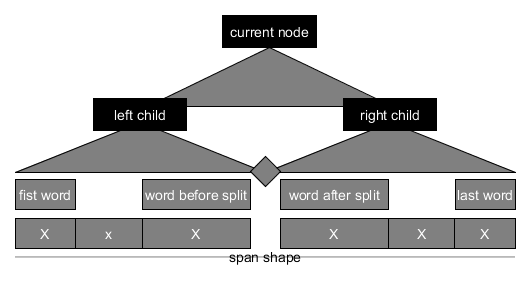
\includegraphics[width=0.7 \textwidth]{spanFeature.png}
	\caption{\label{spanFeature}The span feature from adapted from \cite{ref:2014David}.}
\end{figure*}

\begin{figure}[h!]
	\centering
	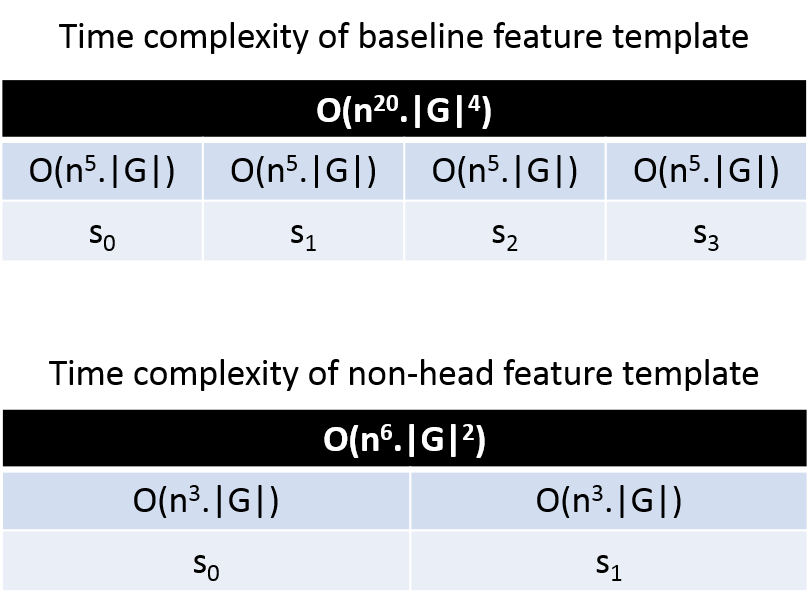
\includegraphics[width=0.45 \textwidth]{FeatureTemplateTimeComplexity.png}
	\caption{\label{featComparison}Comparison of time complexity between baseline and non-head feature template.}
\end{figure}

As in our system, we have designed a feature template which was inspired by the span features in \cite{ref:2014David}. This is a very simple feature set which relied only on the local features within the span of a node and achieve an amazing performace. In the experiment reported in \cite{ref:2014David}, it  has reached an F-score = 89.9\% and outperformed Berkeley parser in terms of parsing many different languages. The span features from this article include the following components for a constituent node (table \ref{simplified subcomp}):
\begin{itemize}
	\item The first and last word of the span of node.
	\item the length of the span of node
	\item The word before and after the split point between left and right child of node.
	\item The shape of word sequence within the span of node (illustrated in figure \ref{spanFeature}):
	\begin{itemize}
		\item X: if the current word's first letter is capital letter.
		\item x: if the current word is normal word.
		\item N: if the current word is a number.
		\item special character such as [' " , .] will remain unchanged.
		\item O: the other cases.
	\end{itemize}
\end{itemize}

\begin{table}
	\caption{\label{simplified subcomp} The sub-components which are used in our simplified feature template}
	\begin{center}
		\begin{tabular}{|l|l|}
			\hline 
			component & explanation \\ 
			\hline
			$X.ft$ &  The first PoS in X's span \\
			$X.fw$ &  The first word in X's span \\
			$X.lt$ &  the last PoS in X's span \\
			$X.lw$ &  the last word in X's span \\
			$X.aSw$ &  The word after-split in X's span \\
			$X.aSt$ &  The PoS after-split in X's span \\
			$X.bSw$ &  The word before-split in X's span \\
			$X.bSt$ &  The PoS before-split in X's span \\
			$X.len$ &  The length of X's span \\
			$X.shape$ &  The shape of X's span \\
			\hline
		\end{tabular}
	\end{center}
\end{table}

Our simplified feature template has been shown in table \ref{simplified feat}. It has focused only on two top nodes in stack $S$($s_0$ and $s_1$) and did not use the head lexical information. Therefore, based on our previous analysis, the time complexity of this feature template will be $O(n^6*|G|^2)$. You can see the illustration of comparison between the baseline and simplified feature template in \ref{featComparison}.

\begin{table*}[t]
	\caption{\label{simplified feat} A table of our simplified feature template}
	\begin{center}
		\begin{tabular}{|l|l|}
			\hline 
			Description & Templates  \\ 
			\hline
			Queue	 	& $q_0.w$+$q_0.t$   ;   $q_1.w$+$q_1.c$   ;   $q_2.w$+$q_2.t$   ;   $q_3.w$+$q_3.c$ \\
			\hline
			$s_0$'s features	 	& $s_0.c$+$s_0.ft$	 ;   $s_0.c$+$s_0.fw$   ;   $s_0.c$+$s_0.lt$   ;   $s_0.c$+$s_0.lw$ \\
			& $s_0.c$+$s_0.aSt$   ;   $s_0.c$+$s_0.aSw$   ;   $s_0.c$+$s_0.bSt$   ;   $s_0.c$+$s_0.bSw$ \\
		    & $s_0.c$+$s_0.ft$+$s_0.lt$   ;   $s_0.c$+$s_0.ft$+$s_0.lw$   ;   $s_0.c$+$s_0.fw$+$s_0.lt$   ;   $s_0.c$+$s_0.fw$+$s_0.lw$ \\
		    & $s_0.c$+$s_0.ft$+$s_0.len$   ;   $s_0.c$+$s_0.fw$+$s_0.len$   ;   $s_0.c$+$s_0.lt$+$s_0.len$   ;   $s_0.c$+$s_0.lw$+$s_0.len$ \\
		    & $s_0.c$+$s_0.ft$+$s_0.lt$+$s_0.len$   ;   $s_0.c$+$s_0.ft$+$s_0.lw$+$s_0.len$ \\
		    & $s_0.c$+$s_0.fw$+$s_0.lt$+$s_0.len$   ;	$s_0.c$+$s_0.fw$+$s_0.lw$+$s_0.len$ \\
			& $s_0.c$+$s_0.len$  ;   $s_0.c$+$s_0.shape$\\
			\hline
			$s_1$'s	features 	& $s_1.c$+$s_1.ft$	 ;   $s_1.c$+$s_1.fw$   ;   $s_1.c$+$s_1.lt$   ;   $s_1.c$+$s_1.lw$ \\
			& $s_1.c$+$s_1.aSt$   ;   $s_1.c$+$s_1.aSw$   ;   $s_1.c$+$s_1.bSt$   ;   $s_1.c$+$s_1.bSw$ \\
			& $s_1.c$+$s_1.ft$+$s_1.lt$   ;   $s_1.c$+$s_1.ft$+$s_1.lw$   ;   $s_1.c$+$s_1.fw$+$s_1.lt$   ;   $s_1.c$+$s_1.fw$+$s_1.lw$ \\
			& $s_1.c$+$s_1.ft$+$s_1.len$   ;   $s_1.c$+$s_1.fw$+$s_1.len$   ;   $s_1.c$+$s_1.lt$+$s_1.len$   ;   $s_1.c$+$s_1.lw$+$s_1.len$ \\
			& $s_1.c$+$s_1.ft$+$s_1.lt$+$s_1.len$   ;   $s_1.c$+$s_1.ft$+$s_1.lw$+$s_1.len$ \\
			& $s_1.c$+$s_1.fw$+$s_1.lt$+$s_1.len$   ;	$s_1.c$+$s_1.fw$+$s_1.lw$+$s_1.len$ \\
			& $s_1.c$+$s_1.len$  ;   $s_1.c$+$s_1.shape$\\
			\hline
		\end{tabular}
	\end{center}
\end{table*}